\section{Literature review method}~\label{rw-tactics-and-topics-for-this-chapter}

Where others have done similar work they've done so in other ways \emph{e.g.} \Gls{msr} and/or \Glspl{slr} rather than focusing on the development teams. While their work is tremendously interesting it does not take the perspective of app developers. Further there is limited prior research that focuses on the use of mobile analytics or effects of analytics on the quality of the mobile apps produced and their related artefacts. 

When I observed the teams the effects of mobile analytics in terms of the processes, artefacts, and the tools emerged. The current characteristics in all three aspects, in: practices, artefacts, and tools led to the realisation that there was a desire to also consider improvements and the effects of those improvements in all three aspects. This led naturally to the 6 perspectives as a three-by-two matrix. 

%\subsection{Notes on the methods used for the literature review} \label{rw-notes-on-methods-used-for-literature-review-topic}

\begin{figure*}
    \centering
    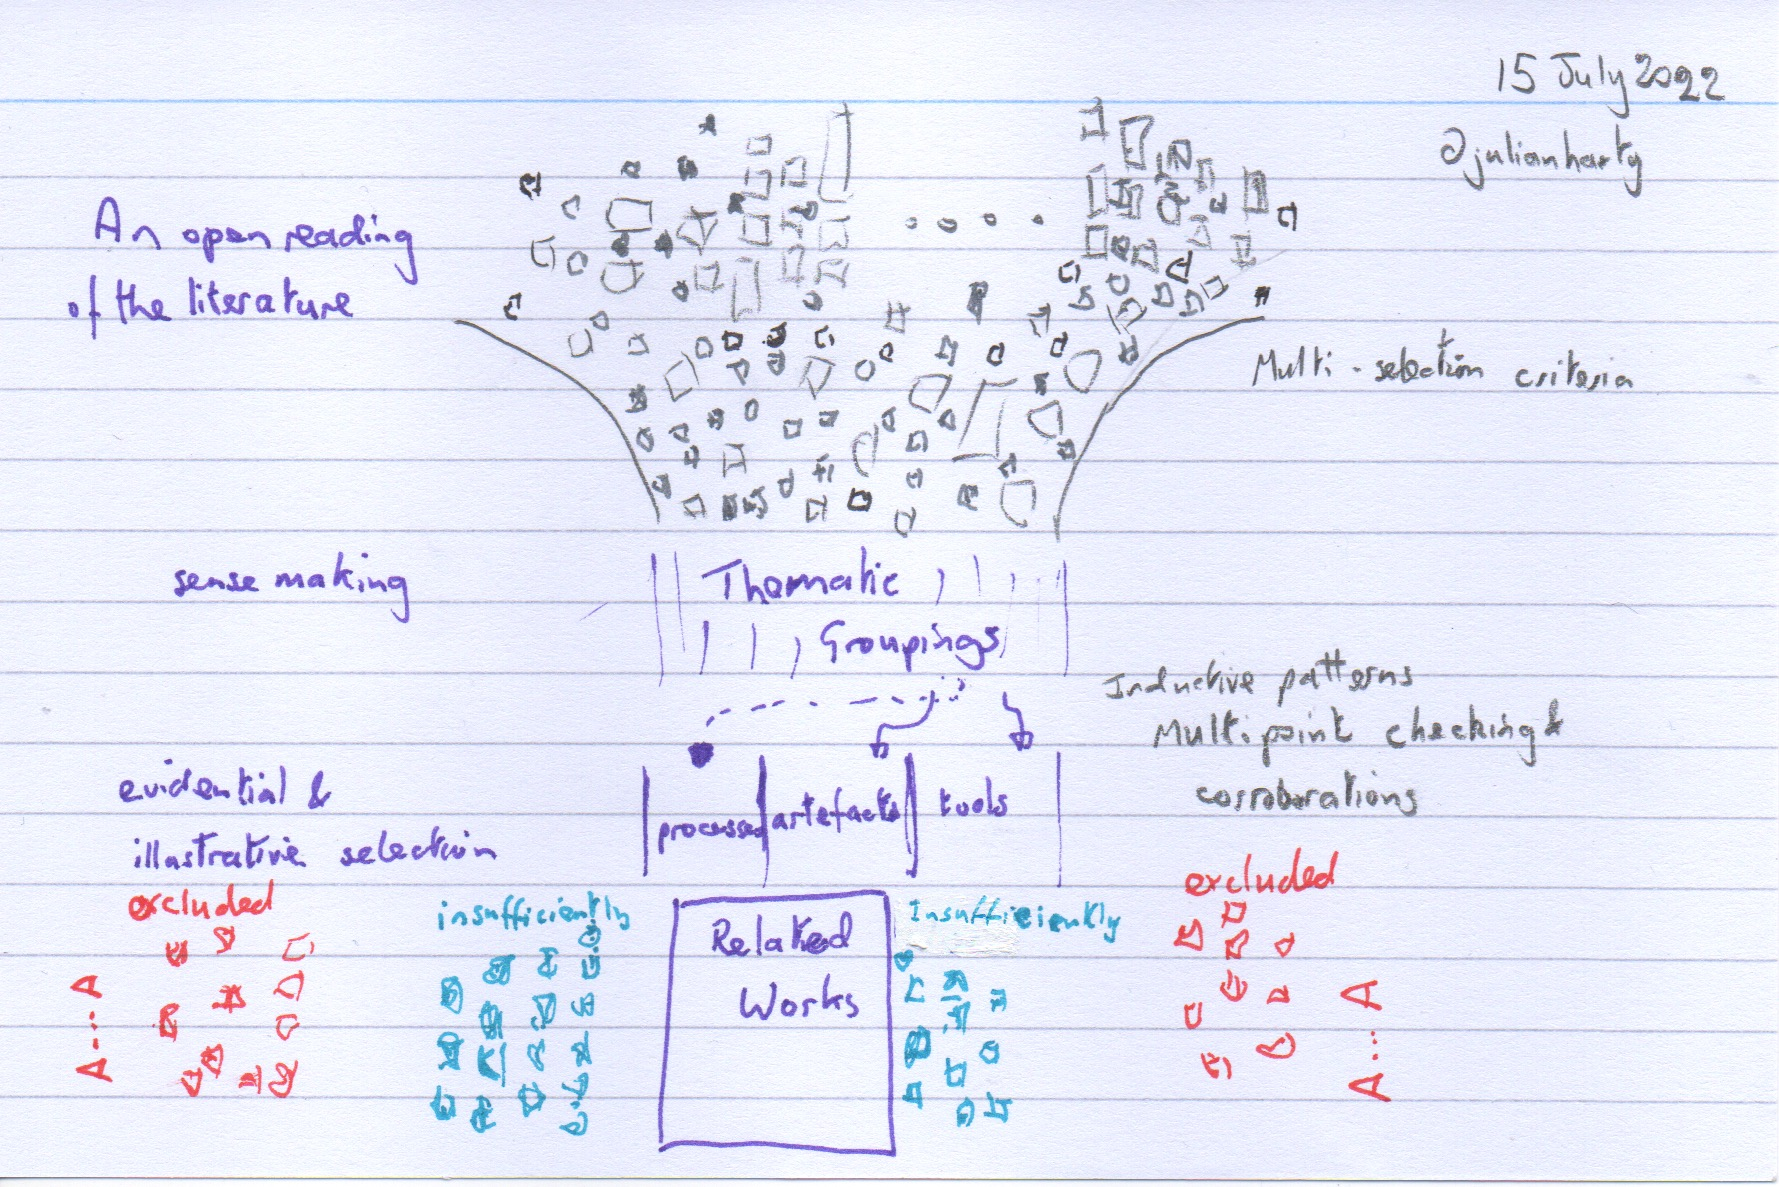
\includegraphics[width=\textwidth]{images/rough-sketches/literature-review-overview.jpeg}
    \caption{Overview of the literature review process and outcomes}
    \label{fig:literature-review-overview}
\end{figure*}

Figure \ref{fig:literature-review-overview} illustrates my approach to researching prior work in the use of mobile analytics by app developers. Various searches, including keyword, tags, and related items, were incorporated into the searches. Many of these searches were inductive, to seek information, patterns, nuggets of research interest, and so on. Other searches were stimulated by events and findings in the case studies.

Initial sources included Google Scholar to find the more research oriented materials and Google Search particularly for grey materials. Specialist search tools were used where sites provided them, for instance on stack exchange sites such as StackOverflow, GitHub.com, acm.org, ieee.org, and medium.com their respective search engines were used frequently. Where practical copies of material has been preserved privately and backed up using at least one commercial, paid-for, cloud file storage service~\sidenote{\emph{i.e.} Dropbox.}.

Multi-selection criteria are used to select material that appears of interest, relevant, and plausible. Generally bibliographic entries were obtained and these where checked for accuracy and completeness. Grey material seldom has a bibliographic entry, these were created by hand, and preserved. Snowball sampling helped increase the breadth of the search results. Termination of searches was based on reaching a point of diminishing returns in terms of new information. Selection was based on relevance to the research and to the case studies.

Through a process of sense-making\index{Sense-making method}, cross-checking, and corroborations, various thematic groupings emerged together with potential relationships between the thematic groups. On reflection three clearly distinct and vital aspects emerged in the related work - the development practices used by mobile app developers, the artefacts they create and maintain, and the mobile analytics tools the developers use. These were further refined into six perspectives, using a three-by-two matrix: the x-axis incorporates the three aspects of processes, artefacts, and mobile analytics tools; the y-axis focuses on the current \emph{what is}, and \emph{what might be} in terms of making improvements. % {Arosha suggested three pillars which sounds good but which I've not managed to apply.}

%The research materials and the bibliographic entries are maintained online. The most relevant ones are included in this thesis, many more are maintained in an `outtakes' folder, for example as `fieldstones'~\sidecite{weinberg2006weinberg} or in an insufficiently-related-works chapter. There's also an `excluded biography' file which helps reduce unnecessary repetition or groundhog day like practices. In the figure (\ref{fig:literature-review-overview}) the two \texttt{A ... A}'s wraps around - excluded works and insufficiently related works are similar distanced to this related works chapter.

In reading the literature various \textit{false friends} emerged, papers that first appear relevant because of their titles and/or abstracts but turn out to be on very different topics. 
Knowing about the concept of false friends and having pragmatic strategies to deal with them is important to avoid misunderstandings or misleading application of their work, 
based on \sidecite[][p. 1833]{chamizodominguez2002_false_friends_their_origins_and_semantics_in_some_languages}. 
% \textcite{shaw1989_comparing_conceptual_structures__consensus_conflict_correspondence_and_contrast} uses the term 'conflict`, where, \emph{``experts use [the] same terminology for different concepts"}~\sidecite[][p. 3]. Shaw and Gaines also discuss false friends  (and, indeed, using their terminology here there is a `correspondence' where experts use two terms to describe the same concept e.g. `false friends' and `conflict' both describe the same concept.). For this research my work was limited to recognising false friends and identifying some examples. 

\begin{comment}
%\subsection{Assessment criteria}~\label{rw-assessment-criteria-topic}
Several areas were used to seed the investigation of the literature. As mobile apps and mobile analytics are both specialisations of broader domains there were likely to be applicable research from the broader domains of software development and software analytics. These provide a research context for the more specialist areas.

%\subsection{Software Quality Improvements for mobile app developers}~\label{rw-software-quality-improvements-for-mobile-app-devs-topic}
Here topics include the measures that have been used by app developers to measure software quality - as confirmed by research literature and grey materials. Sources of information about software quality were included here  (\secref{rw-sources-of-info-on-software-quality-for-devs-of-mobile-apps}).

%\subsection{Development Processes for mobile apps}~\label{rw-devt-processes-for-mobile-apps}
Here topics include how the developers are perceived to work when they develop mobile apps, how they spend their time, how they structure and organise their work, \emph{etc.} Software testing fits here as well as how developers make mobile apps (the artefacts \emph{e.g.} build scripts would go in the artefacts section).

%\subsection{Artefacts for mobile apps}~\label{rw-artefacts-for-mobile-apps}
There's no end of research on artefacts from various subsets of opensource Android projects. Quite how well these reflect the population of shipping mobile apps (in Google Play in particular) is open to discussion. Research into logging practices by developers also fits here (however how they use logging would be part of the section on development processes).

%\subsection{Mobile Analytics (and Mobile Analytics tools)}~\label{rw-mobile-analytics-and-tools-topic}
The research into mobile analytics and mobile analytics tools includes research on the use of mobile analytics and any research into the tools, including the \Glspl{sdk}, data leakage, privacy, etc.

%\subsection{Observations on the organisation of the related works}~\label{rw-thoughts-on-organisation-of-the-rw}
During the literature review there were several instances where a single topic was split across processes and artefacts. An alternative, that might work better, would be to keep the topics together and then summarise the topics by explaining there's a key distinction between the artefacts that exist and how they're used in practice. If so, then the alignment with the six perspectives would occur towards the end of this chapter rather than being used throughout.

    
\end{comment}
